\documentclass[11pt]{article}

\usepackage{fullpage,times}%charter}
\usepackage{color}

\usepackage{tikz}
%\usetikzlibrary{arrows.meta}

%% macros
\newcommand{\ax}[1]{\texttt{AX}(#1)}
\newcommand{\ex}[1]{\texttt{EX}(#1)}
\newcommand{\af}[1]{\texttt{AF}(#1)}
\newcommand{\ef}[1]{\texttt{EF}(#1)}
\newcommand{\ag}[1]{\texttt{AG}(#1)}
\newcommand{\eg}[1]{\texttt{EG}(#1)}
\newcommand{\au}[2]{\texttt{A}(#1\ \texttt{U}\ #2)}
\newcommand{\eu}[2]{\texttt{E}(#1\ \texttt{U}\ #2)}
\newcommand{\sem}[1]{[\!\![#1]\!\!]}

\newcommand{\euntil}[3]{\texttt{E}(#1\ \texttt{U}^{#3}\ #2)}
\newcommand{\auntil}[3]{\texttt{A}(#1\ \texttt{U}^{#3}\ #2)}


\newcommand{\lx}[1]{\texttt{X}(#1)}
\newcommand{\lf}[1]{\texttt{F}(#1)}
\newcommand{\llg}[1]{\texttt{G}(#1)}
\newcommand{\lu}[2]{(#1\ \texttt{U}\ #2)}

%\newcommand{\sol}[1]{{\color{blue}#1}}
\newcommand{\sol}[1]{}
\begin{document}

\hrule
\smallskip

\noindent

\noindent
You can review the latex source for this assignment-file to
learn and use latex to prepare your homework submission. You will see
the use of macros (to write uniformly formatted text), different
text-styles (emphasized, bold-font), different environments (figures,
enumerations).

It is not required that you use exactly this latex source to prepare
your submission. 
\smallskip
\hrule


\begin{center}
{\Large\bf Homework 3 (CTL/LTL/BDD): ComS/CprE/SE 412, ComS 512}

\medskip

Due-date: April 4 at 11:59PM.

\medskip


\end{center}

\noindent
\textbf{
Submit online on Canvas two files: the source file in latex format and
the pdf file generated from latex. Name your files:
$\langle\mbox{your-net-id}\rangle$-hw3.$\langle\mbox{tex/pdf}\rangle$.
}

\hrule
\noindent
\smallskip

\emph{ Homework must be individual's original work. Collaborations and
  discussions of any form with any students or other faculty members
  or soliciting solutions on online forums are not allowed. Please
  review the academic dishonesty policy on our syllabus. If you have
  any questions/doubts/concerns, post your questions/doubts/concerns
  on Piazza and ask TA/Instructor.}

\smallskip
\hrule

\begin{enumerate}

\item For the following Kripke structure with $b\in L(s_3)$, $\{a, b\}\subseteq L(s_2)$, $a\in L(s_1)$ and
  $b\in L(s_4)$,
        \begin{center}
    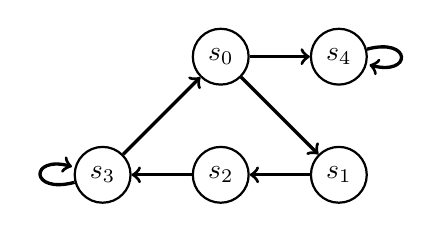
\begin{tikzpicture}

      \begin{scope}[every node/.style={circle,thick,draw}]
        \node (s0) at (1.5,1.5) {$s_0$};
        \node (s1) at (3,0) {$s_1$};
        \node (s2) at (1.5,0) {$s_2$};
        \node (s3) at (0,0) {$s_3$};
        \node (s4) at (3,1.5) {$s_4$};p
      \end{scope}

      \begin{scope}[%>={Stealth[black]},
          every node/.style={fill=white,circle},
          every edge/.style={draw=black,very thick}]
        \path [->] (s0) edge (s4);
        \path [->] (s0) edge (s1);
        \path [->] (s1) edge (s2);
        \path [->] (s2) edge (s3);
        \path [->] (s4) edge[loop right] (s4);
        \path [->] (s3) edge (s0);
        \path [->] (s3) edge[loop left] (s3);
      \end{scope}
    \end{tikzpicture}
        \end{center}
 We are given a function defined as follows:
        \[
        A_{\varphi}(Z) = \sem{\varphi}_M \ \cap\ R_{\forall}(R_{\forall}(Z))
        \]
 where $\varphi$ is some CTL formula, $\sem{\varphi}_M$ is the
 semantics of $\varphi$ (in the context of a Kripke structure $M = (S,
 T, L)$ ) defined as a set of states of a Kripke structure, and
 $R_{\forall}$ is
        \[
        R_{\forall}(Z) = \{s~|~\forall s'. (s, s') \in T \ \Rightarrow \ s' \in Z\}
        \]
 \begin{enumerate}
 \item Compute the greatest fixed point $A_{b}$ for the given Kripke structure.
 
\textbf{Answer:}

$R_{\forall}(Z) = \{ s_0, s_1, s_2, s_3, s_4\} = Z$, therefore, $R_{\forall}(R_{\forall}(Z)) = Z$ and $\sem{b}_M = \{s_2, s_3, s_4\}$

\[ A_{b}(Z) = \sem{b}_M \ \cap\ R_{\forall}(R_{\forall}(Z))  = \{ s_2, s_3, s_4\} \cap \{ s_0, s_1, s_2, s_3, s_4\}  = \{ s_2, s_3, s_4\}\]

\[ A^2_{b}(Z) = \sem{b}_M \ \cap\ R_{\forall}(R_{\forall}(A_{b}(\{ s_2, s_3, s_4\})))  = \{ s_2, s_3, s_4\} \cap \{ s_0, s_1, s_4\}  = \{ s_4\}\]

\[ A^3_{b}(Z) = \sem{b}_M \ \cap\ R_{\forall}(R_{\forall}(A^2_{b}(\{ s_4\})))  = \{ s_2, s_3, s_4\} \cap \{s_4\}  = \{ s_4\}\]

\[ A^4_{b}(Z) = \sem{b}_M \ \cap\ R_{\forall}(R_{\forall}(A^3_{b}(\{s_4\})))  = \{ s_2, s_3, s_4\} \cap \{ s_4\}  = \{ s_4\}\]
\[ \vdots \]

Therefore, the greatest fixed point of $A_{b}(Z) =  \{ s_4\}$. 


 
 \item \textbf{512 only} It is claimed that the semantics
   of the property expressed by the greatest fixed point of
   $A_{b}$ cannot be expressed in CTL. Justify the validity of
   the claim.
   
\textbf{Answer:} 

If we look at $R_{\forall}(R_{\forall}(\{ s_2, s_3, s_4\}))$ for $A^2_{b}(Z)$, we get, $R_{\forall}(\{ s_2, s_3, s_4\}) = \{ s_1, s_2, s_4\}$ and $R_{\forall}(R_{\forall}(\{ s_2, s_3, s_4\})) = \{ s_0, s_1, s_4\}$. Therefore, $R_{\forall}(R_{\forall}(\{Z\}))$ captures next states of next states of current state satisfying the properties given in the question. This implies the greatest fixed points capture all the even states starting from $s_4$. However, all states starting from $s_4$ satisfies $b$, but the fixed points only capture the even states starting from $s_4$. 

Therefore, it cannot be expressed in CTL. 
   
 \end{enumerate}
\hfill (6+4(Extra Credit))
 

\item
  Your company requires that in any collaborative project, code commits
  must be reviewed by collaborator(s) of the person who commits the
  code.  One fine morning, you wake up to see your collaborator has
  committed some late night code written in Pseudo-Lang with minimal
  comments. Your job is to review the commit and provide some
  constructive comments.

  The only code-comments are as follows:
  \begin{itemize}
  \item The code utilizes ROBDD implementation where each node of the
    ROBDD is described using a structure \emph{node} containing three
    properties: \emph{name} of the decision variable for that node;
    a pointer to the root of the left-subtree (\emph{left}); and
    a pointer to the root of the right-subtree (\emph{right}).

    The terminal or leaf nodes are associated with the \emph{name}
    true or false (and have null pointers for \emph{left} and
    \emph{right}).

  \item The code corresponds to some function with two formal
    parameters each of type node, and returns a boolean type.

    \end{itemize}

\begin{verbatim}
function wit(struct node n1, struct node n2) {
   if ((n1.name == true) && (n2.name == false)) return true;
   if ((n2.name == true) && (n1.name == false)) return true;
   if ((n1.left == null) || (n2.left == null)) return false;
   if (n1.name == n2.name) {
      if (wit(n1.left, n2.left))
          return wit(n1.right, n2.right)
      }
   return false;
}
\end{verbatim}

\begin{enumerate}
\item What is the functionality of the function \emph{wit}?

\textbf{Answer}: It checks if two ROBDDs having the same set of decision nodes are inverse of each other, which means their terminal nodes are opposite of each other. 


\item What is the runtime of the function \emph{wit}?

The function's runtime is equal to the exponential size of ROBDD. 

%we can write it as $2^{S}$ where S is the size of ROBDD. 

\end{enumerate}
\hfill (10)

\item
  For each of the following requirements, discuss whether LTL and CTL
  model checking can be used to verify the requirements. For instance,
  if your answer for some requirement is: it can be verified using LTL
  model checking but not using CTL model checking, then justify your
  answer. 
  \begin{enumerate}
  \item Along all paths, propositions $p$ and $q$ hold true in alternate
    states.
    
\textbf{Answer}: 
    This is expressible in both CTL and LTL. 

    CTL : $ (p \lor q) \land \ag{ (p \rightarrow \ax{q}) \land (q \rightarrow \ax{p})}$

    LTL : $(p \lor q) \land \llg{ ( p \rightarrow \lx{q}) \land (q \rightarrow \lx{p})}$

    Therefore, it is verifiable in both LTL and CTL. 

    
    
  \item Along all paths, eventually a state is reached such that all
    its next states satisfy the proposition $p$.

 
\textbf{Answer}: This can be expressed in CTL but not in LTL because LTL cannot capture branching behavior after reaching a state. The CTL formula satisfying the requirement is $\af{\ax{p}}$. Therefore, CTL model checking can be used to verify this property. 
    
  \item There exists no path where $p$ holds true until $q$ holds true.

\textbf{Answer}: This can also be represented in both LTL and CTL. 

CTL: $\neg \au{p}{q}$ 

LTL: $\neg \lu{p}{q}$

So, both LTL and CTL model checking can be used to verify this property. 


  \item There exists a path where $p$ holds in a state and it is followed
    by a state where $q$ holds.

    \textbf{Answer}:  

    CTL representation of this formula: $\ef{p \land \ex{q}}$. 


    
    The statement's negation becomes "For all paths, $p$ holds in a state, and it is not followed by a state where $q$ holds", or we can also write negation as "For all paths, $p$ does not holds in a state, and it is not followed by a state where $q$ holds" and so on. 
        
        It is evident that even if we negate the expression, the branching behavior remains.  
    Therefore, it is expressible and verifiable in CTL but cannot be expressed and verified in LTL.

    
    \end{enumerate}
\hfill(12)
  

\item Prove or disprove the following claims:
  \begin{enumerate}
  \item For any path $\pi$ in a Kripke structure, $\pi \models
    \lu{\lf{p}}{q}$ and $\pi[0]$ does not satisfy $q$ implies that
    there must be some state(s) where $p$ holds true before the state
    where $q$ holds true.

    \textbf{Answer}: \textit{disproved}, \textit{Explanation}: Assume a path $\pi = s_0s_1s_2s_3...$, $\pi[0] \not \models q $, and $ \pi \models \lu{\lf{p}}{q}$. 
    This implies $\pi[0] \models \lf{p}$, and a path can satisfy $\lf{p}$ if p becomes true at anywhere in the path for some $i\geq 0$. Therefore,  $\pi \models \lu{\lf{p}}{q}$ does not demand $p$ be true in states before $q$. 

    Let's elaborate it as 

     $\pi \models \lu{\lf{p}}{q}$ iff $\exists i. \pi^i \models q \land \forall j < i. \pi^j \models \lf{p}$

     Now let's consider path starting from $\pi^j$ ,  $\pi^j \models \lf{p}$ iff $\exists k \geq 0. \pi^k \models p$   

    Here, $k$ value might be greater than $i$, and still $\pi^j \models \lf{p}$ is satisfied. 
    
   Therefore, this statement is incorrect.

    
    
\item For any state in any Kripke structure, the state satisfies
  $\ax{\af{p}}$ if and only if the same state satisfies $\lf{\lx{p}}$.

\textbf{Answer}: \textit{proved}, \textit{Explanation}: This is vacuously true. $\ax{\af{p}}$ implies for all paths starting from all next states of the current state, it is possible to eventually reach $p$. The equivalent LTL formula is $\lx{\lf{p}}$. $\lx{\lf{p}}$ is equivalent to  $\lf{\lx{p}}$.

For the following Kripke structure TS with $p\in L(s_1)$, $\{p\}\subseteq L(s_3)$ and $s_0$ as the initial state. 
        \begin{center}
    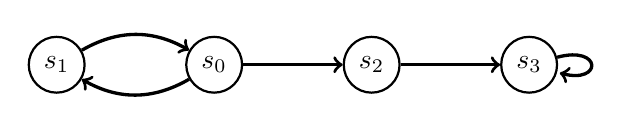
\begin{tikzpicture}

      \begin{scope}[every node/.style={circle,thick,draw}]
        \node (s0) at (0,0) {$s_0$} ;
        \node (s1) at (-2,0) {$s_1$};
        \node (s2) at (2,0) {$s_2$};
        \node (s3) at (4,0) {$s_3$};
      \end{scope}

      \begin{scope}[%>={Stealth[black]},
          every node/.style={fill=white,circle},
          every edge/.style={draw=black,very thick}]
        \path [->] (s0) edge[bend left, above] (s1);
        \path [->] (s0) edge (s2);
        \path [->] (s1) edge[bend left, below] (s0);
        \path [->] (s2) edge (s3);
        \path [->] (s3) edge[loop right] (s3);

      \end{scope}
    \end{tikzpicture}
        \end{center}

Here, $TS \models \ax{\af{p}}$ and it also satisfies the LTL formula $TS \models \lx{\lf{p}}$. 



\item The LTL formula $\lf{\llg{p}} \Rightarrow \llg{\lf{p}}$ is
    equivalent to propositional constant true. 

\textbf{Answer}: \textit{proved}, \textit{Explanation}: 

$\lf{\llg{p}} \Rightarrow \llg{\lf{p}}$ can be written as $\neg (\lf{\llg{p}}) \lor \llg{\lf{p}}$ = $\llg{\lf{ \neg p}} \lor \llg{\lf{p}}$

Which is a tautology. Therefore, $\lf{\llg{p}} \Rightarrow \llg{\lf{p}}$ is equivalent to propositional constant true. 


    
    \end{enumerate}
\hfill(12)
  
\end{enumerate}


\end{document}

